

\subsection{Spieldesign}



\subsubsection{Allgemeines} Am Anfang der Entwicklung musste ein geeignetes Setting für das geplante RPG gefunden werden. Zur Auswahl standen die beiden klassischen, den meisten bekannten Arten von Spieleuniversen. Die eine wäre futuristische Science Fiction und die andere eher mittelalterliche Fantasy. 

In der frühen Phase der Entwicklung war beim Spieldesign ursprünglich geplant ein RPG zu entwickeln, dass viele Elemente des klassischen Pen-and-Paper Rollenspiels, wie z.B. Dungeons \& Dragons enthält. Man wollte unterschiedliche Charakterklassen, die sich in ihrer Ausrüstung, wie individuellen Waffen und Rüstungen, sowie ihren spezifischen Fähigkeiten, klar voneinander unterscheiden. Ein Levelsystem, bei dem die einzelnen Charaktere von Abenteuer zu Abenteuer ihre Fähigkeiten verbessern und bessere Ausrüstung in Form von Beutegut finden können, sollte auch enthalten sein. Das Entwicklerteam hat sich dann für das Fantasy-Setting entschieden, weil man der Ansicht war, dass sich die vorher genannten Eigenschaften damit besser umsetzen lassen. Speziell die unterschiedlichen Eigenschaften der Charakterklassen waren bei dieser Entscheidung maßgeblich. Denn eine Eingrenzung auf die besonderen Fähigkeiten der unterschiedlichen Spielfiguren, wie z.B. Tank, Heiler und Damagedealer, schien im Science Fiction-Setting nicht so einfach und für den Spieler nicht schlüssig zu gestalten.

\begin{figure}[H]
    \centering
    \caption{Details den Klassen aus der Projektbesprechung vom 11.12.2021}
    \label{fig:2021-12-11-Projekt-Besprechung-Klassenbeschreibung}
    \fbox{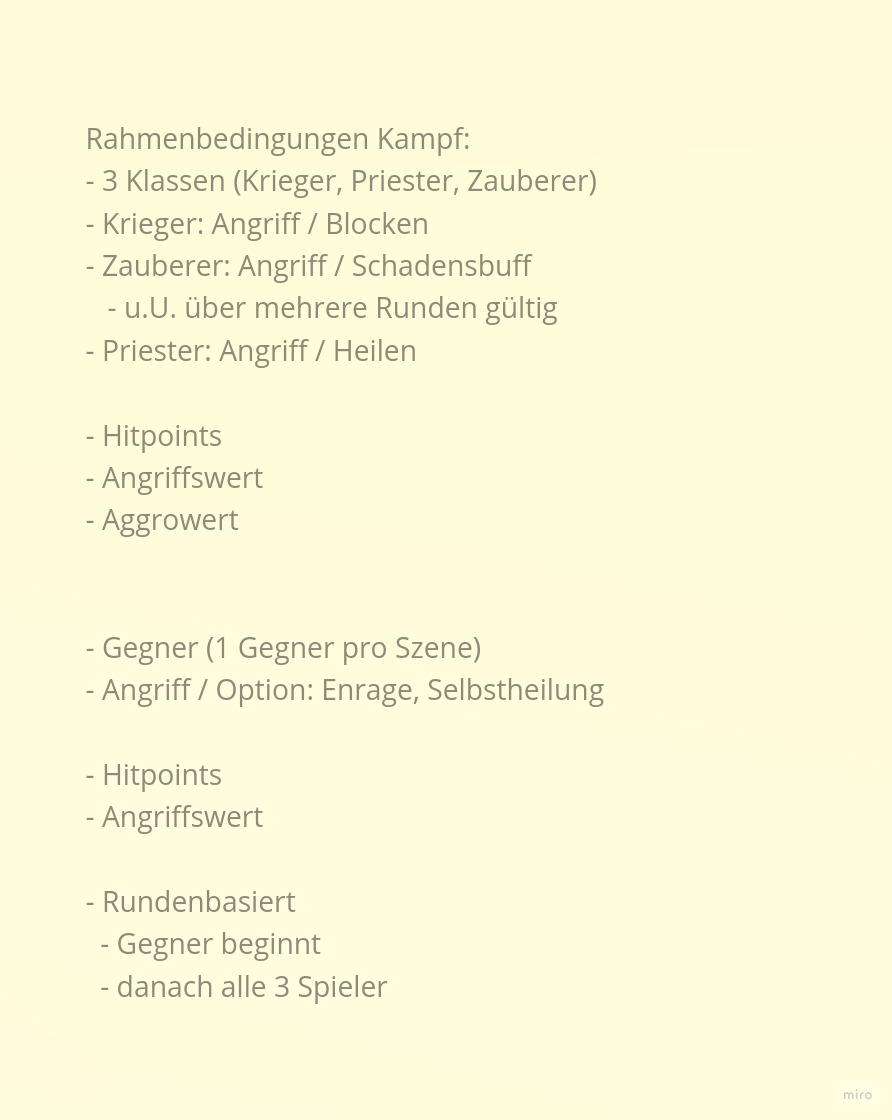
\includegraphics[width=0.4\textwidth]{2021-12-11-Projekt-Besprechung-Klassenbeschreibung}}
\end{figure}


Die Überlegungen führten somit schon am Anfang recht schnell zu den bereits erwähnten unterschiedlichen Spielfiguren, die der Spieler verkörpern kann. Ein Tank soll Schaden von anderen und sich selbst abhalten können. Ein Heiler soll sich und seine Mitspieler heilen können. Ein Damagedealer soll seinen Schaden und den der anderen Spielfiguren erhöhen. Es war angedacht, dass die einzelnen Spielfiguren über Lebenspunkte, Magiepunkte und verschiedene Handlungsoptionen verfügen, die sich, abhängig von der Charakterklasse, voneinander unterscheiden. Auch schien klar zu sein, dass die Würfelmechanik, die Pen-and-Paper Rollenspielen zu Grunde liegt, in das Spiel übernommen werden soll.

Das Spiel sollte vom Ablauf her, aus aufeinander aufbauenden Abenteuern bestehen, die die Charaktere gemeinsam erleben und die mit Hilfe von unterschiedlichen Ansätzen gelöst werden können, bestehen. Dazu sollten sie sich gemeinsam durch eine grafisch animierte Spielwelt bewegen.

Es sollte Regeln geben, die bestimmen wie und in welcher Reihenfolge der Kampf abläuft oder zu welchen Bedingungen z.B. ein Schwerthieb trifft. Dies sollte auf Grundlage der Open Source Lizenz des Rollenspiels Dungeons \& Dragons 3.5 basieren.

Nachdem dieser grobe Rahmen festgelegt wurde, entschieden wir zunächst einmal einen Prototypen zu entwickeln, der die grundlegende technische Machbarkeit unserer Ideen beweisen sollte.

Dabei fiel recht schnell auf, dass vor allem die geplanten Unterschiede der einzelnen Charakterklassen, in Form von sich unterscheidenden Handlungsmöglichkeiten in der Szene, nicht klar abzugrenzen sind. Außerdem war nicht klar, wie es zu handhaben ist, wenn der Charakter z.B. vor einer verschlossenen Tür steht und jede Klasse eine andere Möglichkeit hat dieses Hindernis zu überwinden. 

Bei diesem Beispiel ist recht einfach zu klären, wie die unterschiedlichen Handlungsmöglichkeiten aussehen könnten: "Tür eintreten", "Schloss knacken" und "Tür mit Magie öffnen". Dabei war allerdings nicht klar, wie genau dies ablaufen sollte. Wer z.B. darf in diesem Moment die Handlung bestimmen? Derjenige, der zuerst auf den Button klickt? Und was geschieht danach, entsprechend der unterschiedlichen Auswahl der Möglichkeiten? Sollte jede Aktion zu unterschiedlichen Ergebnissen führen oder zu denselben? Dieses würde wiederum die Auswahl, was zu tun ist, völlig unnötig machen. Und falls die Auswahl zu unterschiedlichen Ergebnissen führt, entsteht ein für uns nicht einzuschätzender Aufwand an Storytelling, grafischen Animationen und an Programmierarbeit. Außerdem ist die Komplexität der Kampfmechanik, wie sie in dem Regelsystem von Dungeons \& Dragons 3.5 geregelt ist, recht anspruchsvoll und für einen gemütlichen Abend mit seinen Freunden und auf das Spielen von Angesicht zu Angesicht ausgelegt. Dies ermöglicht eine andere Spielweise als allein vor einem PC. Zum Beispiel kann sich ein Charakter aus dem Kampf zurückziehen oder ein anderer aus der Abenteurergruppe nimmt seinen Platz in der Kampflinie ein. Der Spielleiter, der die Gegner steuert, kann auch entscheiden einen anderen Charakter anzugreifen, wenn er den Eindruck hat, dass der Charakter sonst stirbt. Dies sind  Mechaniken, die zwar zu programmieren möglich sind, aber den Rahmen für das erste Projekt dieser Art sicher sprengen würden.
Außerdem besteht ein Charakter in diesem Regelwerk aus vielen Eigenschaften, die in Zahlenwerten festgehalten werden. All diese Werde beeinflussen wie er z.B. kämpfen, stehlen oder mit anderen Menschen interagieren kann. Jeder Gegenstand, der als Beutegut von den Charakteren gefunden wird, hat Auswirkungen darauf. Dies ist nur eine grobe Zusammenfassung der Dinge, die die Regelmechanik beeinflussen. Auch große Spieletitel wie z.B. \textit{Baldur's Gate} von BioWare, die ebenfalls auf Dungeons \& Dragons 3.5 basieren, haben nicht das gesamte Regelwerk übernommen. 

Aufgrund all der oben genannten Unwägbarkeiten und Komplexität, haben wir uns an diesem Punkt zu einer im Folgenden erklärten Konzeptänderung entschieden.

Der gravierendste Schritt ist sicher, dass aus dem RPG-Adventure ein stärker auf Kämpfe ausgerichtetes Rollenspiel mit Fantasy-Setting und atmosphärischen Texten und Grafiken geworden ist. Dabei gibt es zwar noch immer einzelne Level, die man durchspielt, diese sind aber recht linear und bestehen nur aus einem Kampf gegen einen Gegner. Ganz grob soll es wie folgt ablaufen:

Am Anfang der Szene wird ein Introbild mit Ambienttext eingeblendet und nachdem die oder der Spieler bestätigt haben, wechselt die Ansicht. Nun sieht man eine Abbildung der Szene mit dem Gegner. Rechts davon befindet sich das Kampflog links darunter die Charakteranzeige und ganz unten das Chatfenster. Je nach Ausgang des Kampfes wird ein anderer Outrotext angezeigt und man springt zurück auf die Weltkarte. Es wird keine Ausrüstung geben, die die Charaktere finden können, denn jeder gefundene Gegenstand sollte unterschiedliche Eigenschaften haben und sich in irgendeiner Weise auf den Charakter auswirken. Dies hätte zu diesem Zeitpunkt der Entwicklung zu einem zu umfangreiches Datenbankmanagement geführt. Das Konzept, dass ein Charakter seine Eigenschaften verbessert, in dem er bei den Kämpfen an Erfahrung gewinnt, besteht weiterhin, wenn auch etwas einfacher als zunächst angedacht. Auch ist es so geblieben, dass sich jede Charakterklasse von der anderen durch eine Spezialfähigkeit unterscheidet. Die Klassen sind ebenfalls geblieben, nur hat sich die Bezeichnung etwas konkretisiert. Im Einzelnen sind das der Krieger, der die Möglichkeit hat den erhaltenen Schaden zu reduzieren. Dann gibt es noch den Priester, der die Fähigkeit hat zu Heilen, während der Magier den Schaden erhöhen kann. Nach jedem Kampf gibt eine individuelle Summe an Erfahrung, die dem Charakter gutgeschrieben wird. Diese kann er dazu benutzen die Fähigkeiten seines Charakters zu verbessern. Der Spieler kann mit der erhaltenen Erfahrung die Lebenspunkte (HP) oder die Angriffskraft (AP) seines Charakters steigern. Ein Charakter erhält immer Erfahrung, egal ob der Kampf gewonnen wird oder verloren geht. Bei einem Sieg ist diese jedoch deutlich höher als bei einer Niederlage. Das hat zur Folge das man einen Level eventuell mehrfach spielen muss, um den nächsten Level erfolgreich abschließen zu können. Der Mechanismus des Würfelns ist ebenfalls in der Art implementiert, dass nicht jeder Treffer einen festen Schaden zufügt, sondern es einen Minimum- und einen Maximumschaden gibt, der zufällig zwischen beiden Extremen errechnet wird. Der endgültige Tod eines Charakters ist nicht vorgesehen. 

Die Kampfmechanik wird wie folgt aussehen: Der Kampf ist deutlich vereinfacht und wird rundenbasiert ablaufen, wobei in jeder Runde der Gegner zuerst angreift. Danach wird jeder Charakter die Möglichkeit haben entweder anzugreifen oder seine Spezialfähigkeit einzusetzen. Aussetzen ist ebenfalls möglich. Falls der Charakter seine Spezialfähigkeit nutzt, kann er nicht angreifen und umgekehrt. Die Spezialfähigkeit wirkt mehrere Runden nach. Es ist nicht vorgesehen zu testen, ob ein Angriff trifft oder nicht, ein Angriff trifft also immer und macht Schaden. Der Gegner verfügt über keine Spezialfähigkeiten. Macht dieser Schaden, so wird ein Spieler ausgewählt, dem dann der spezifischen Schaden zugefügt wird. D.h. der Warg der z.B. 20 Punkte Schaden pro Angriff macht, fügt dem ausgewählten Charakter die 20 Punkte Schaden zu. Der Schaden der Spieler summiert sich, sodass drei Spieler, die jeweils 20 Schaden zufügen, dem Warg in Summe 60 Punkte Lebensenergie abziehen. Vor jedem neuen Kampf verfügen die Spieler wieder über ihre vollen Lebenspunkte (HP).

\subsubsection{Balancing} Trotz der recht einfachen Mechanik ist das Balancing doch recht komplex. Die einzelnen Klassen unterscheiden sich klar in ihren Fähigkeiten voneinander und sollen trotz ihrer unterschiedlichen Spielweise ungefähr gleichwertig sein und dem Spieler natürlich auch gleich viel Spaß bereiten. Um dafür die richtigen Stellschrauben zu haben, sind sämtliche Werte so hinterlegt, dass sie einzeln abgeändert werden können. Im Einzelnen stellt sich das wie folgt dar: 

Wie schon erwähnt, können HP und AP für jede Klasse und jeden Gegner einzeln und völlig unabhängig voneinander abgeändert werden. Die Spezialfähigkeiten der einzelnen Charakterklassen sind in Dauer und Ausprägung unterteilt, die sich wie bei den anderen Werten individuell für jede Klasse einzeln regeln lassen. Auch die erhaltene Erfahrung ist mit einem abänderbaren Multiplikator versehen, um Einfluss darauf zu nehmen, wie viel Erfahrung die einzelnen Charaktere erhalten und wie schnell sie ihre Fähigkeiten verbessern können. Dabei ist ebenfalls darauf geachtet worden, dass es die Möglichkeit gibt, dass HP und AP unterschiedlich viele Erfahrungspunkte kosten können und wie alle anderen Werte ist dies auch variabel einstellbar. Die unterschiedlichen Erfahrungspunktkosten von HP und AP sind nötig, weil der Unterschied von diesen die Charaktere voneinander abgrenzt und diese im Kampf unterschiedlich wichtig sind und die Spieler nicht zu schnell zu mächtig werden sollen.

\begin{lstlisting}
"name": "ability_m_effect_strength",
"type": "float", "value": "0.6",
"hint": "strength of the mage ability in percent (written in float, 0.1 = 10%, 0.5 = 50%)"

"name": "ability_m_duration_rounds",
"type": "int", "value": "2",
"hint": "mage ability will be applyed to this number of next rounds"

"name": "ability_p_effect_strength",
"type": "float", "value": "0.08",
"hint": "strength of the priest ability in percent (written in float, 0.1 = 10%, 0.5 = 50%)"

"name": "ability_p_duration_rounds",
"type": "int", "value": "4",
"hint": "priest ability will be applyed to this number of next rounds"

"name": "ability_w_effect_strength",
"type": "float", "value": "0.20",
"hint": "strength of the warrior ability in percent (written in float, 0.1 = 10%, 0.5 = 50%)"

"name": "ability_w_duration_rounds",
"type": "int", "value": "3",
"hint": "warrior ability will be applyed to this number of next rounds"
\end{lstlisting}

Die Trennung von HP und AP hat außerdem zur Folge, dass nicht jeder Charakter derselben Klasse demselben Stereotyp entspricht. Also ist es möglich, dass sich jeder Krieger, so der Spieler denn möchte, anders entwickeln kann als der Krieger, den der Spieler davor gespielt hat. Der Spieler kann also einen Krieger erschaffen, der entweder Wert auf HP oder AP legt und das jedes Mal individuell neu entscheiden. Dies gilt auch für alle anderen Klassen. Der variable Schaden soll dazu dienen, dass nicht jeder Kampf vorherberechnet werden kann, indem man die HP des Gegners mit den AP des Spielers vergleicht.

All das führt dazu, dass das Balancing gut und kleinschrittig angepasst werden kann, macht es aber aufgrund der vielen Stellschrauben auch sehr komplex und für uns, die wir über wenig Erfahrung im Spielebalancing verfügen, auch schwierig alles aufeinander abzustimmen. Die im veröffentlichten Spiel festgelegten Werte stellen einen Kompromiss aus Arbeitsaufwand und Spielbarkeit bzw. Spielerfahrung dar. Diese könnten noch durch ein umfangreiches Beta-Testing, das üblicherweise an so einem Punkt bei Spieleentwicklungen geschieht, optimiert werden. Dafür gibt es hier aber weder Zeit noch Ressourcen, um die Rückmeldungen von einer Vielzahl von Testern auszuwerten und in die Entwicklung einfließen zu lassen und anschließend nochmals zu Prüfen ob die Änderungen zu den gewünschten Ergebnissen geführt haben. Beim Balancing des Spiels hat sich außerdem gezeigt, dass die Teilbereiche Programmierung und Balancing unbedingt eng zusammenarbeiten sollten. So kann sichergestellt werden, dass die nötigen Mechaniken auch vorhanden sind und nicht noch nachträglich evtl. umständlich implementiert werden müssen. Wenn dies dann überhaupt noch möglich ist.

\subsubsection{Storytelling} Am Anfang war generell festzulegen in welcher Sprache das Spiel erscheinen soll, dabei standen Englisch und Deutsch zur Auswahl. Ursprünglich sollte das Spiel auf Englisch erscheinen und die ersten Konzepttexte der Charakterbeschreibungen wurden auch in englischer Sprache verfasst (zu sehen in folgender Abbildung). 

\begin{figure}[H]
    \centering
    \caption{Entwurfszeichnung und Text für eine Charaktererstellungsseite (29.11.2021)}
    \label{fig:2021-11-29-Entwurf-Klassen-Ui}
    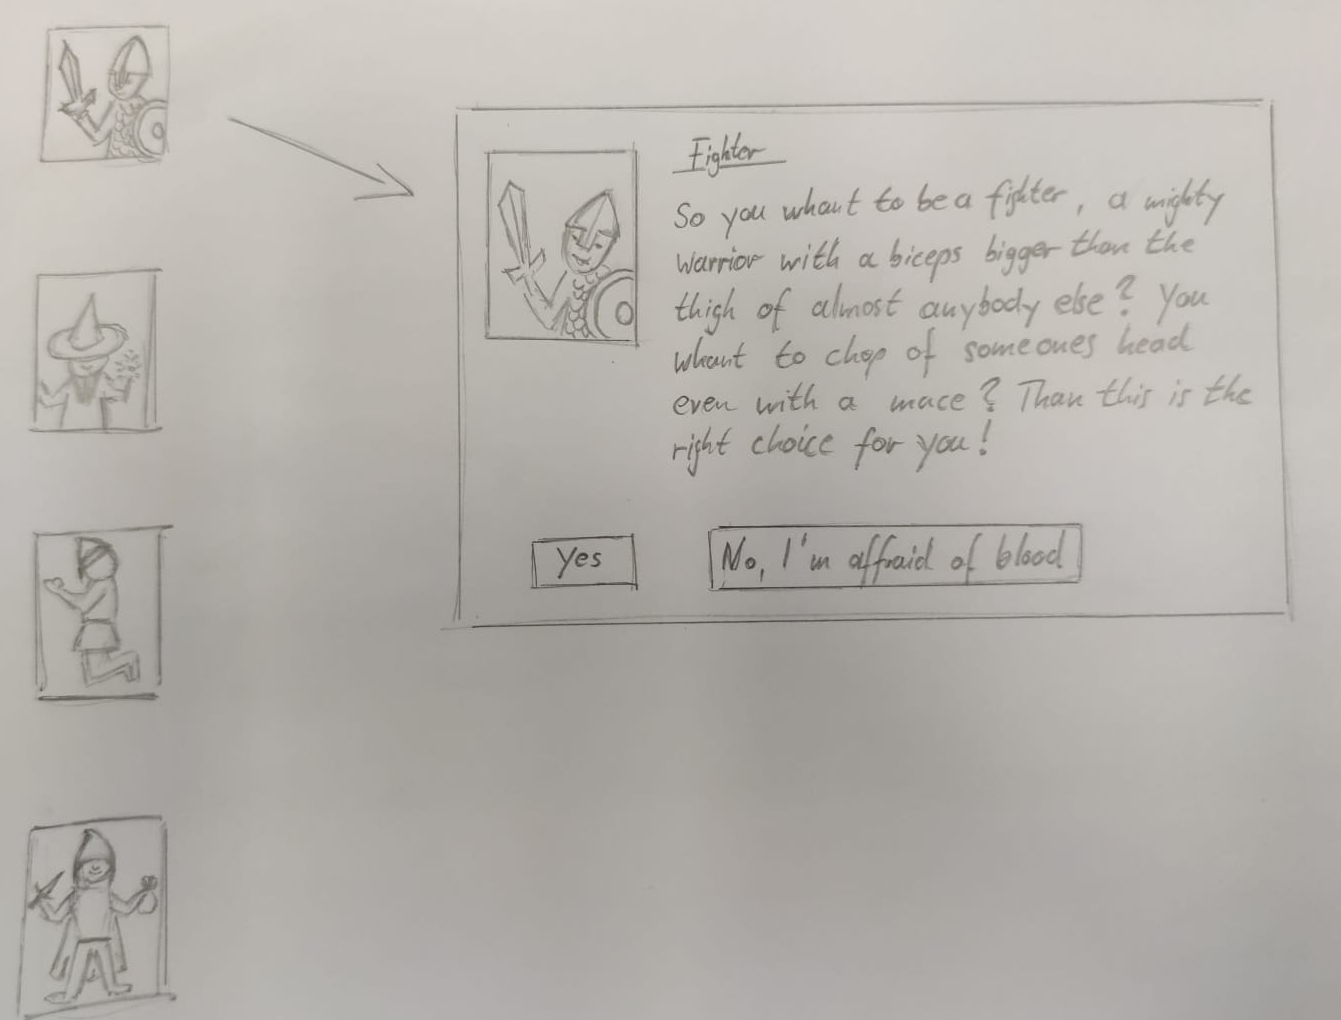
\includegraphics[width=0.7\textwidth]{2021-11-29-Entwurf-Klassen-Ui}
\end{figure}

Da allerdings jeder der Projektteilnehmer deutscher Muttersprachler ist, wurde die Projektsprache Deutsch festgelegt. Außerdem wird das Spiel nur im Zusammenhang eines Studienprojektes entwickelt und soll im deutschsprachigen Raum veröffentlicht werden. Um die Entwicklung nicht unnötig auf Grund von sprachlichen Schwierigkeiten zu verkomplizieren, schien dieser Schritt logisch. 

Die Entwicklung hin zu einem Spiel, in dem die Level oder Spielszenen nur lose zusammenhängen, machte es nötig zu jeder einzelnen Szene eine Story zu schreiben, um dem Spieler ein Gefühl zu geben, was gerade passiert und warum. Außerdem sind unterschiedliche Texte je nach Ausgang der Spieleszene vorgesehen und Texte, die z.B. beschreiben was gerade im Kampf geschieht. Dabei ist es wichtig sich auf die Beschreibung der dargestellten Szene zu konzentrieren und nicht abzuschweifen, da ein zu langer Text vom Spieler vielleicht nicht gelesen oder als störend empfunden wird. Jedoch muss er lang und intensiv genug sein, damit sich der Spieler einen Eindruck von dem Geschehen verschaffen und darin eintauchen kann. Schließlich soll das Spiel auch eine Geschichte erzählen und dem Spieler eine gewisse Spielerfahrung und im Idealfall einen Wiederspielwert geben. 

Beim Entwickeln der einzelnen Szenen ist aufgefallen, dass man nicht immer genau sagen kann, was zuerst da war, das Huhn oder das Ei, denn der Text und die Grafik stehen in engem Zusammenhang und haben sich gegenseitig beeinflusst. Die Beschreibung der Szene stand üblicherweise zuerst und danach wurde die Szenengrafik entwickelt. Aber manchmal war es auch umgekehrt oder es war nötig den Text anzupassen, weil die Animation z.B. eines Rudels Wölfe schwieriger war als die von einem einzigen riesigen Wolf. So wurde aus dem Rudel Wölfe, das die Gegend terrorisiert, ein einzelner großer Warg. Oder im Fall der Szene im Anwesen war bei ursprünglicher Planung ein Geist als Gegner vorgesehen, aber beim Schreiben der Geschichte wurde daraus ein Vampir, der viel düsterer ist und besser passt.

Daraus ist abzuleiten, dass bei einer Spieleentwicklung diese beiden Teilbereiche sehr eng zusammenarbeiten sollten. Für den Programmierer z.B. ist es egal, was für eine Grafik oder Text an entsprechender Stelle im Code eingefügt werden soll. Oder um es in den Worten unserers Lead-Programmers auszudrücken: "Ich bin da total leidenschaftslos". Aber Spiel- und Grafik-Design müssen unbedingt Hand in Hand gehen und sich gegenseitig ergänzen, um eine überzeugende Spielerfahrung zu schaffen. 

Im Fall des Kampfes gegen den Drachen und den Vampirlord ist man bewusst von der reinen Beschreibung der Szene abgewichen und hat viel mehr die Motivation des Charakters und etwas Hintergrundgeschichte in den Vordergrund gestellt, um beim Spieler die Beweggründe des Charakters in den Vordergrund zu stellen. So kann sich dieser, nicht wie bei den anderen Szenen in die Handlung, sondern mehr in den Akteur selbst hineinversetzen. Bei diesen Gegnern sollte auch etwas Besonderes im Text stehen, außerdem wollte der Autor auch unterschiedliche Arten der Erzählung ausprobieren.
